\section{Comparator Design and Analysis}

The comparator circuit is the location where the digital decision is made. It detects the polarity of a differential analog input signal and generates a digital output (1 or 0) accordingly or compares a SE input to a threshold (reference) voltage.

\subsection{Two-Stage OTA Comparator}
As shown in Figure 5.1, the comparator is based on two stage 5T OTA with high gain or high slope between input and output. So, if $Vin + > Vin -$ the output is \textit{VDD}. Conversely, if $Vin - > Vin +$ the output is ground. This comparator has high performance and low voltage offset with higher gain but consumes high biasing current with high power consumption.

\begin{figure}[h]
    \centering
    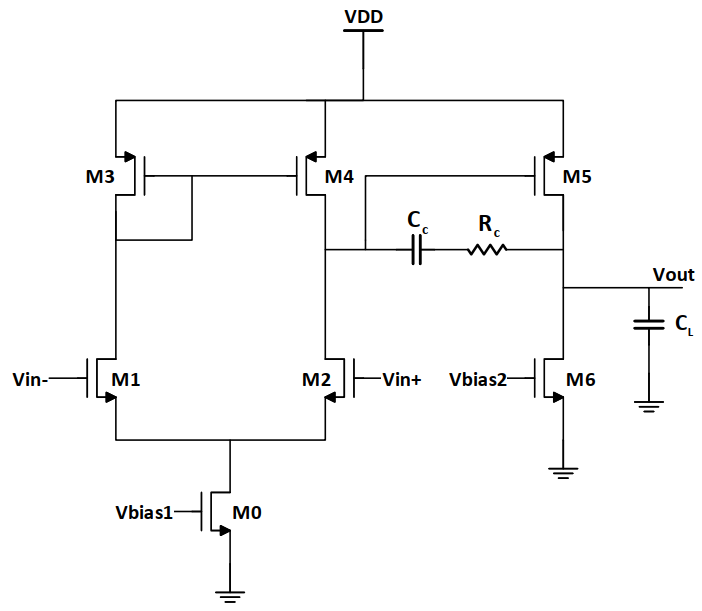
\includegraphics[width=0.5\textwidth]{img/DFE_img/DFE_img_26.png}
    \caption{Two-Stage OTA}
\end{figure}

\subsection{The Strong-Arm Latch}
The Strong-Arm (SA) latch is a dynamic comparator widely used for its zero static power consumption and full rail-to-rail output swing. The latch of Figure 5.2 consists of a clocked differential pair, M1-M2, two cross-coupled pairs, M3-M4 and M5-M6, tail transistor Q7and four pre-charge switches, S1--S4. The circuit provides rail-to-rail outputs at outp and outn in response to the polarity of \textit{Vin}1 \textit{- Vin}2.

\subsubsection*{Phases of Operation}

1. \textbf{Reset Phase (CLK=0):} The tail transistor MT is OFF. Pre-charge transistors pull internal nodes P, Q, and output nodes (X, Y) to VDD.

2. \textbf{Amplification Phase (CLK=1):} M7 turns ON and the four switches are OFF. M3-M6 are initially off. The input differential pair discharges nodes P and Q making differential urrent depends on the input voltage. This phase provides voltage gain until either $V_P$ or $V_Q$ is ON. This time called $t_A$ where it equals:

\begin{equation}
    t_A \approx \frac{C_{Q,P} V_{thn}}{I_{CM}} 
\end{equation}

Voltage gain equals:

\begin{equation}
    V_P - V_Q = V_{id} \cdot \frac{t_A}{C_{P,Q}} \cdot {gm}_{1,2} \quad (\text{where } A = \frac{t_A}{C_{P,Q}} \cdot {gm}_{1,2}) 
\end{equation}

\begin{equation}
    A = \frac{2I_{CM}}{V_{CM} - V_{th,n}} * \frac{C_{Q,P}V_{th,n}}{I_{CM}} * \frac{1}{C_{Q,P}} = \frac{2V_{thn}}{V_{CM} - V_{th,n}} 
\end{equation}

Or $A = \frac{{gm}_{1,2}V_{thn}}{I_{CM}}$ (5.3)

When P \& Q falls below $V_{DD} - V_{thn}$ M3 \& M4 begin to operate. Nodes P, Q keep discharging and $V_{OUT +}$, $V_{OUT -}$ start discharging differently according to the unbalance of P and Q. $V_{OUT +} - V_{OUT -} \approx AV_{id}$. Gain plays an important role for reducing noise and offsets comes from cross coupled M3-M6.

3. \textbf{Regeneration Phase:} When Vout+ or Vout- goes lower than Vdd-|Vthp|, one between M5 and M6 turns on:

If Vout- hits first, M5 turns on, and Vout+ is pulled towards Vdd (M6 is off)M4 is more "conductive" allowing Vout- to lower. M2 eventually enters linear region.M3 progressively turns off due to lowering Vout-. Hence it cuts the M5-M3 DC path \textbf{(no static power).} \textbf{It is positive feedback loop (regeneration).}

\begin{equation}
    G_R = \exp{\left(\frac{t_2 - t_1}{\tau_R}\right)} 
\end{equation}

(Assuming M1/M2 in linear region) (where $t_1$ is when PMOS is open and $t_2$ is the decision time)

\begin{equation}
    \tau_R = \frac{C_{out}}{{gm}_{5,6} + {gm}_{3,4}} 
\end{equation}

\begin{figure}[h]
    \centering
    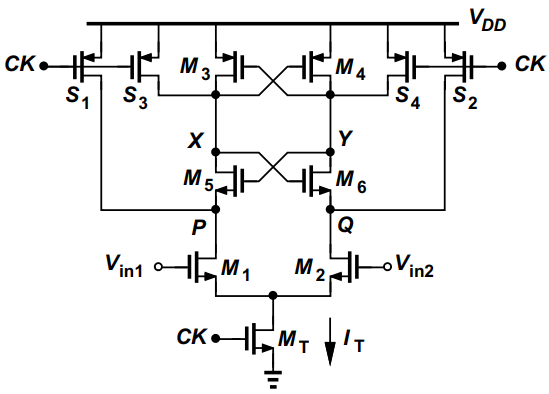
\includegraphics[width=0.5\textwidth]{img/DFE_img/DFE_img_27.png}
    \caption{Strong Arm Latch}
\end{figure}

\subsubsection*{Limitations}

- \textbf{Input common mode voltage variations:} Gain and $t_A$ are dependent on $V_{CM}$. So, there is an optimum input common mode voltage to give least delay and if it shifts, we will have variations in delay which is bad for DFE.

I have simulated Strong Arm and swept for input common mode voltage using those sizing:

\begin{table}[h]
    \centering
    \begin{minipage}{0.48\textwidth}
        \centering
        \begin{tabular}{|c|c|c|}
            \hline
            \textbf{Transistor} & \textbf{Length} & \textbf{Width} \\
            \hline
            M1, M2 & 22nm & 8um \\
            \hline
            M3, M4 & 22nm & 2.4um \\
            \hline
            M5, M6 & 22nm & 2.4um \\
            \hline
            M7 & 22nm & 4um \\
            \hline
        \end{tabular}
        \caption{Transistor Sizing for Strong Arm Latch}
    \end{minipage}
    \hfill
    \begin{minipage}{0.48\textwidth}
        \centering
        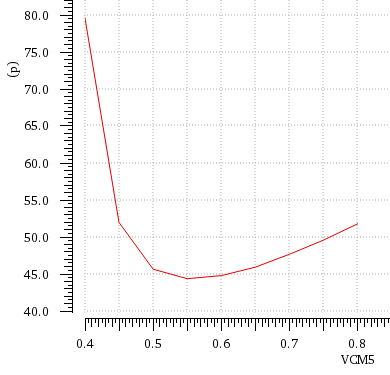
\includegraphics[width=.9\textwidth]{img/DFE_img/DFE_img_28.png}
        \caption{Input common mode variation}
    \end{minipage}
\end{table}

- \textbf{Kickback Noise:} The "kickback" currents drawn from the inputs stem from several mechanisms exhibiting both differential and CM components.
 $V_P$ and $V_Q$ fall toward ground at unequal rates and couple to the inputs through $C_{GD1}$ and $C_{GD2}$ causing diff kickback noise. 
 The CM kickback noise currents are much greater and occur when M7 turns on, initially drawing its drain current from $C_{GS1}$ and $C_{GS2}$, 
 and when it turns off, with CK coupling through $C_{GD7}$ to $C_{GS1}$ and $C_{GS2}$.

\begin{figure}[h]
    \centering
    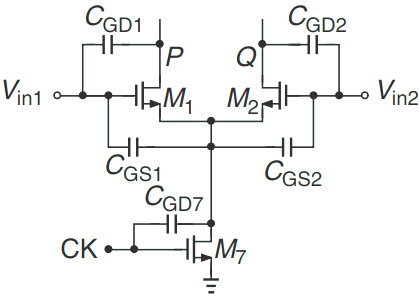
\includegraphics[width=0.4\textwidth]{img/DFE_img/DFE_img_29.png}
    \caption{Kickback Noise}
\end{figure}

- \textbf{Offset:} In a typical design, the mismatches between M3 and M4 are divided by about a factor of $A_v \approx 4$ when referred to the input, and those between M5 and M6 by about a factor of ten (because these transistors turn on only near the end). Thus, M1 and M2 become the dominant contributors.

- \textbf{Input referred noise:} M1 and M2 are the dominant contributors and as the gain increases the contributions of M3-M6 becomes less.

\subsection{The Double-Tail Latch}
To mitigate the limitations of the Strong-Arm latch, the \textbf{Double-Tail Latch} separates the circuit into two distinct stages: an input stage and a latching stage.

\subsubsection*{Advantages}
\begin{itemize}
    \item \textbf{Voltage Headroom:} By separating the stages, the transistor stacking is reduced (typically 3 transistors in stack vs. 4 in SA). This allows operation at lower supply voltages (VDD).
    \item \textbf{Independent Optimization:} The input stage can be optimized for low noise and low offset (large devices, small current), while the second stage is designed for speed (small devices, high current).
    \item \textbf{Reduced Kickback:} The inter-stage nodes isolate the regeneration nodes from the input, significantly reducing differential kickback noise.
    \item \textbf{Non sensitive to variation in input common mode voltage:} due to separation of input stage from latching stage. Each has its own current, so $V_{icm}$ doesn't affect much as Strong Arm.
\end{itemize}

\begin{figure}[h]
    \centering
    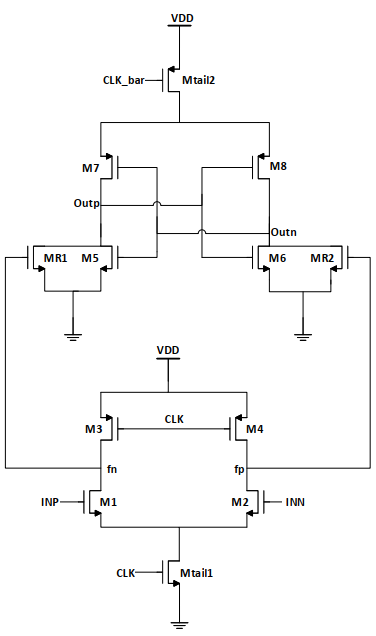
\includegraphics[width=0.35\textwidth]{img/DFE_img/DFE_img_30.png}
    \caption{Double Tail Latch}
\end{figure}

\newpage
\subsection{CML Latch}
CML is faster but has static current which consumes more power than Strong Arm

- \textbf{At the sampling phase:}

\begin{equation}
    Vout(0) = Gm1 \times RD \times Vin 
\end{equation}

- \textbf{At the regeneration phase:}

\begin{equation}
    Gm3 \times Vout = \frac{Vout}{RD} + CL \frac{dVout}{dt}
\end{equation}

\begin{equation}
    Vout(t) = Gm1 \times RD \times Vin \exp{\left( \frac{Gm3 \times t}{CL} \right)} \exp{\left( \frac{-t}{RD \times CL} \right)} 
\end{equation}

Where Gm3 must be greater than $\frac{1}{RD}$

\begin{figure}[h]
    \centering
    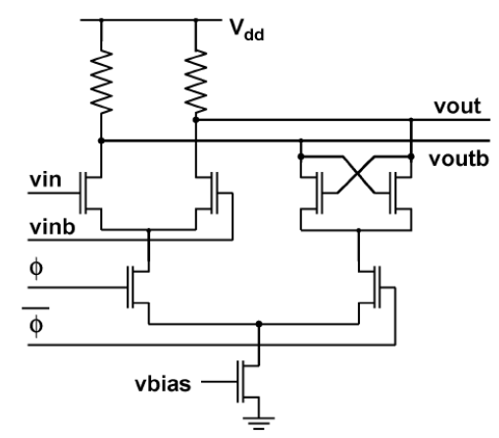
\includegraphics[width=0.4\textwidth]{img/DFE_img/DFE_img_31.png}
    \caption{CML Latch}
\end{figure}

\subsection{Comparison: SA vs. CML}
Current-Mode Logic (CML) latches are faster and offer higher bandwidth but consume static power.

\begin{itemize}
    \item \textbf{Bandwidth:} Strong-Arm latches generally have higher sampling bandwidth than CML latches.
    \item \textbf{Gain:} CML latches provide higher sampling gain, especially with small input devices.
\end{itemize}

To form a Flip-Flop:
\begin{itemize}
    \item After strong-arm latch, cascade an R-S latch
    \item After CML latch, cascade another CML latch
\end{itemize}

Strong-Arm flip-flop has the advantage of no static power dissipation and full CMOS output levels

\subsection{SR Latch}
To keep data for the whole clock period it is required to implement SR Latch after Strong Arm to keep the data but it adds delay to the delay of Latch. So, it required to implement fast SR Latch.

\subsubsection*{Conventional SR Latch}

\begin{figure}[h]
    \centering
    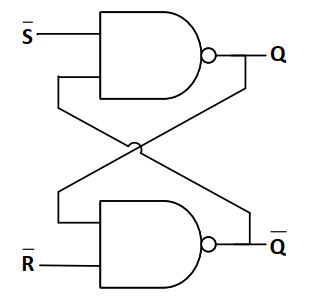
\includegraphics[width=0.25\textwidth]{img/DFE_img/DFE_img_32.png}
    \caption{SR Latch}
\end{figure}

The low level at both \textit{S} and \textit{R} node is not permitted and that is guaranteed by the SA stage. The low level at \textit{S} sets the \textit{Q} output to high, which in turn forces \textit{Q} to low. Conversely, the low level at \textit{R} sets \textit{Q} the high, which in turn forces \textit{Q} to low. Therefore, one of the output signals will always be delayed with respect to the other. The rising edge always occurs first, after one gate delay, and the falling edge occurs after two gate delays. This limits the performance of the SAFF (Strong Arm Flip-Flop).

\subsubsection*{Improved SR Latch}
As shown in Fig 5.6. The SR latch is modified in order to overcome the problem of the SR latch in SAFF.

\begin{equation}
    Q^{+} = S + \overline{R}Q 
\end{equation}

\begin{equation}
    \overline{Q^{+}} = R + \overline{S}Q 
\end{equation}

M1, M4, M7, M10 represents drivers

M2, M5, M9, M12 represents keepers

In reset phase the drivers are off and the keepers are ON making the cross-coupled inverters M3, M6, M8, M11 are ON also which keeps the previous value.

In evaluation phase, the keepers are OFF and the drivers sets the output of SR Latch.

\begin{figure}[h]
    \centering
    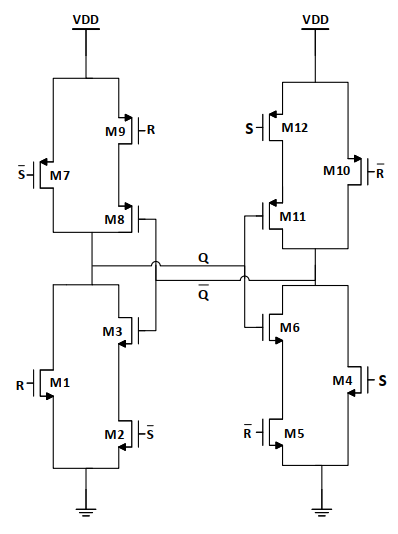
\includegraphics[width=0.35\textwidth]{img/DFE_img/DFE_img_33.png}
    \caption{Improved SR Latch}
\end{figure}

\subsection{Offset Cancellation}
As offset contributes much in errors. It should be calibrated to minimize the erros

\subsubsection*{Offset Cancellation using capacitors}
Using capacitors to make voltage difference opposes the voltage difference caused by mismatch

\begin{equation}
    V_{OS,in} = \left(\frac{I_{SS}}{2{gm}_{1,2}}\right) \left(\frac{C_P}{C_Q} - 1\right) 
\end{equation}

\begin{figure}[h]
    \centering
    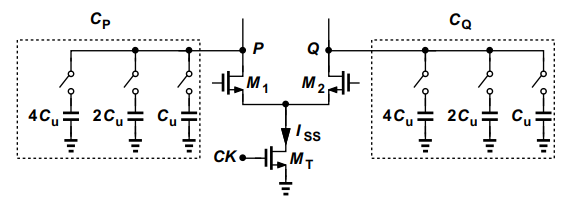
\includegraphics[width=0.6\textwidth]{img/DFE_img/DFE_img_34.png}
    \caption{Offset Cancellation}
\end{figure}

Adjust $C_P$ \& $C_Q$ until offset is cancelled. This method degrades speed and increase power consumption $( = fC{V_{DD}}^{2})$. Also consumes large area.

\subsubsection*{Self Calibrating Offset}
Voltage offset cancellation is done by using two NANDs and charge pump. The comparator offset voltage becomes less than ±1 LSB ( = Ts × Icp / CH ). The gate of MC1 is connected to Vb to set the common mode voltage of the charge pump.

\begin{figure}[h]
    \centering
    \begin{minipage}{0.48\textwidth}
        \centering
        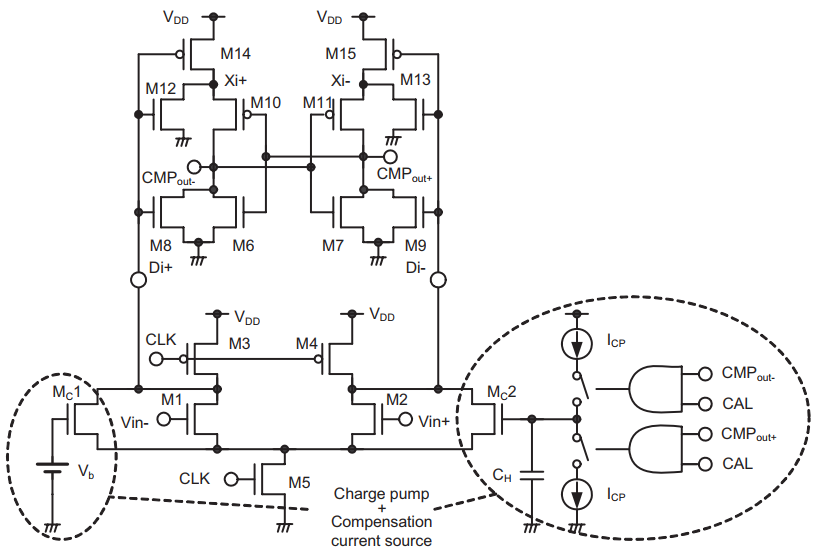
\includegraphics[width=\textwidth]{img/DFE_img/DFE_img_35.png}
    \end{minipage}
    \hfill
    \begin{minipage}{0.48\textwidth}
        \centering
        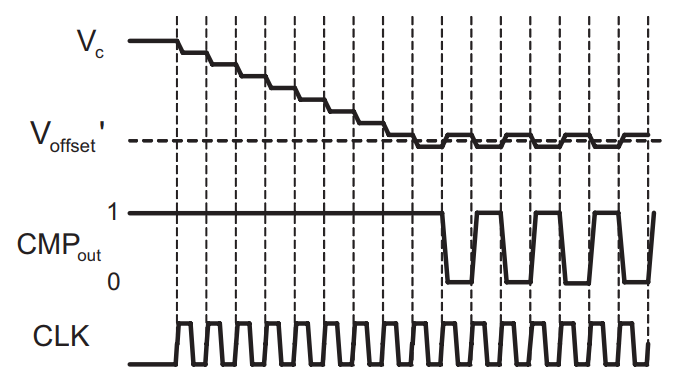
\includegraphics[width=\textwidth]{img/DFE_img/DFE_img_36.png}
    \end{minipage}
    \caption{Proposed architecture for offset cancellation \cite{miyahara2008}}
\end{figure}